% Thesis chapter: training the regression and scoring BC policies, and their differences.
% Standalone chapter file; \input or \include from the thesis root.
% Requires graphicx; figures live in figures/ relative to this file.
% Sources: scripts/envs/train_bc_pointcloud.py (regression),
%          scripts/envs/scoring_head.py + train_scoring_head.py (scoring),
%          scripts/envs/summarize_noise_sweep.py (degradation sweep),
%          real_trials.ods + render_policy_comparison.py (field trials).

\chapter[Learning Grasp Selection from Point Clouds]{Learning Grasp Selection from Point Clouds: Regression and Scoring Policies}
\label{ch:bc_policies}

This chapter describes the two behavior-cloned grasp policies used on the crane:
a \emph{regression} policy that maps the observed point cloud directly to grasp
coordinates, and a \emph{scoring} policy that scores every observed point and
grasps at the highest-scoring one. Both are trained by supervised learning on
the same expert demonstrations and share the same PointNet feature trunk; they
differ only in how the grasp is parameterized and, consequently, in the loss
that supervises it. That difference determines their behavior: the regression
policy minimizes a mean-squared error and therefore averages over multimodal
expert behavior, while the scoring policy minimizes a classification loss over
observed points and is mode-seeking by construction. Section~\ref{sec:bc_common}
covers the shared data pipeline, Sections~\ref{sec:bc_regression} and
\ref{sec:bc_scoring} the two policies, and Section~\ref{sec:bc_differences}
makes the differences explicit. Section~\ref{sec:bc_trials} closes the loop
with field trials on the physical crane: a three-trial baseline campaign whose
failure analysis motivated the scoring design, offline replays of both
policies on the recorded failure clouds, a simulated observation-degradation
sweep, and two hardware trials of the scoring policy itself.

\section{Common Setup: Demonstrations, Observations, and Labels}
\label{sec:bc_common}

\subsection{Expert demonstrations}

Demonstrations are collected in simulation from a privileged expert that reads
ground-truth log poses. At each grasp cycle the expert selects the topmost log
in the rack, targets its center, and computes the grapple yaw that aligns the
grapple with the log's long axis. Executing this expert clears piles reliably,
so the dataset records one tuple per successful grasp cycle:
\begin{equation}
  \mathcal{D} = \big\{ (P_k,\; t_k,\; \psi_k) \big\}_{k=1}^{M},
\end{equation}
where $M$ is the number of recorded cycles,
$P_k \in \mathbb{R}^{N \times 3}$ is the point cloud observed at the
start of the cycle, $t_k = (t_x, t_y, t_z) \in \mathbb{R}^3$ is the commanded
grasp center in the crane base frame, and $\psi_k$ is the commanded grapple
yaw. Because the expert targets log \emph{centers}, the label height satisfies
$t_z = z_{\mathrm{surf}} - r_{\log}$ by construction, where
$z_{\mathrm{surf}}$ is the local pile surface and $r_{\log} = 0.056$~m is the
log radius. This identity is what later allows relabeling to a different
digging depth (Section~\ref{sec:bc_dig}).

Piles are randomized between episodes. The final collection recipe spawns
profiled piles (localized mounds with randomized amplitude, width, and
multi-bump structure, plus per-log scale jitter) and truncates episodes after a
small number of grasp cycles so that mound-shaped, informative states dominate
the dataset rather than the flat late-episode remainders.

\subsection{Observation pipeline}

The observation is a simulated depth-camera point cloud processed by
Algorithm~\ref{alg:obs_pipeline}, the same procedure the deployed node runs.
The raw camera cloud is transformed into the crane
base frame, cropped to an axis-aligned box around the rack, and downsampled
with farthest-point sampling (FPS) to a fixed budget of $N$ points ($N = 1024$
for the tight-crop datasets, $N = 2048$ for the widened-crop datasets):
\begin{equation}
  P = \mathrm{FPS}_N\!\left( \mathrm{crop}_{[b^{\min} - m,\; b^{\max} + m]}
      \left( T_{\mathrm{base} \leftarrow \mathrm{cam}} \, P_{\mathrm{raw}} \right) \right).
\end{equation}
Here $[b^{\min}, b^{\max}]$ is the action box, the volume of commandable grasp
centers,
\begin{equation}
  b^{\min} = (-5.364,\; -1.684,\; -1.30), \qquad
  b^{\max} = (-3.364,\; 5.316,\; 0.10) \quad [\mathrm{m}],
\end{equation}
and $m$ is an optional crop margin. The tight datasets use $m = 0$ (the
observation crop equals the action box); the margin datasets use $m = 0.5$~m
in $x$ and $y$, so the policy also sees context immediately outside the box
(bed apron, rack posts) while the set of commandable grasps is unchanged.
Clouds with fewer than $N$ points after cropping are zero-padded, and both
policies mask padded slots explicitly.

The margin exists because of a sim-to-real asymmetry, illustrated in
Figure~\ref{fig:bc_sim_vs_real_crop}. In simulation the tight crop removes
the bed plane, the rack rails, and the pole columns, so a tight-crop policy
trains on clouds that contain logs and nothing else. On the real crane those
surfaces intrude into the same crop volume: rack ends, pole columns, and the
bed remain visible, and late in a trial, once the pile drops below the rail
height, they become the most prominent geometry in the crop. A policy trained
on the tight crop therefore never sees, at training time, the structure it is
most likely to mis-target at deployment. Widening the observation crop and
spawning the corresponding structure in simulation restores parity between
what the network trains on and what it will be shown.

\begin{figure}[t]
\centering
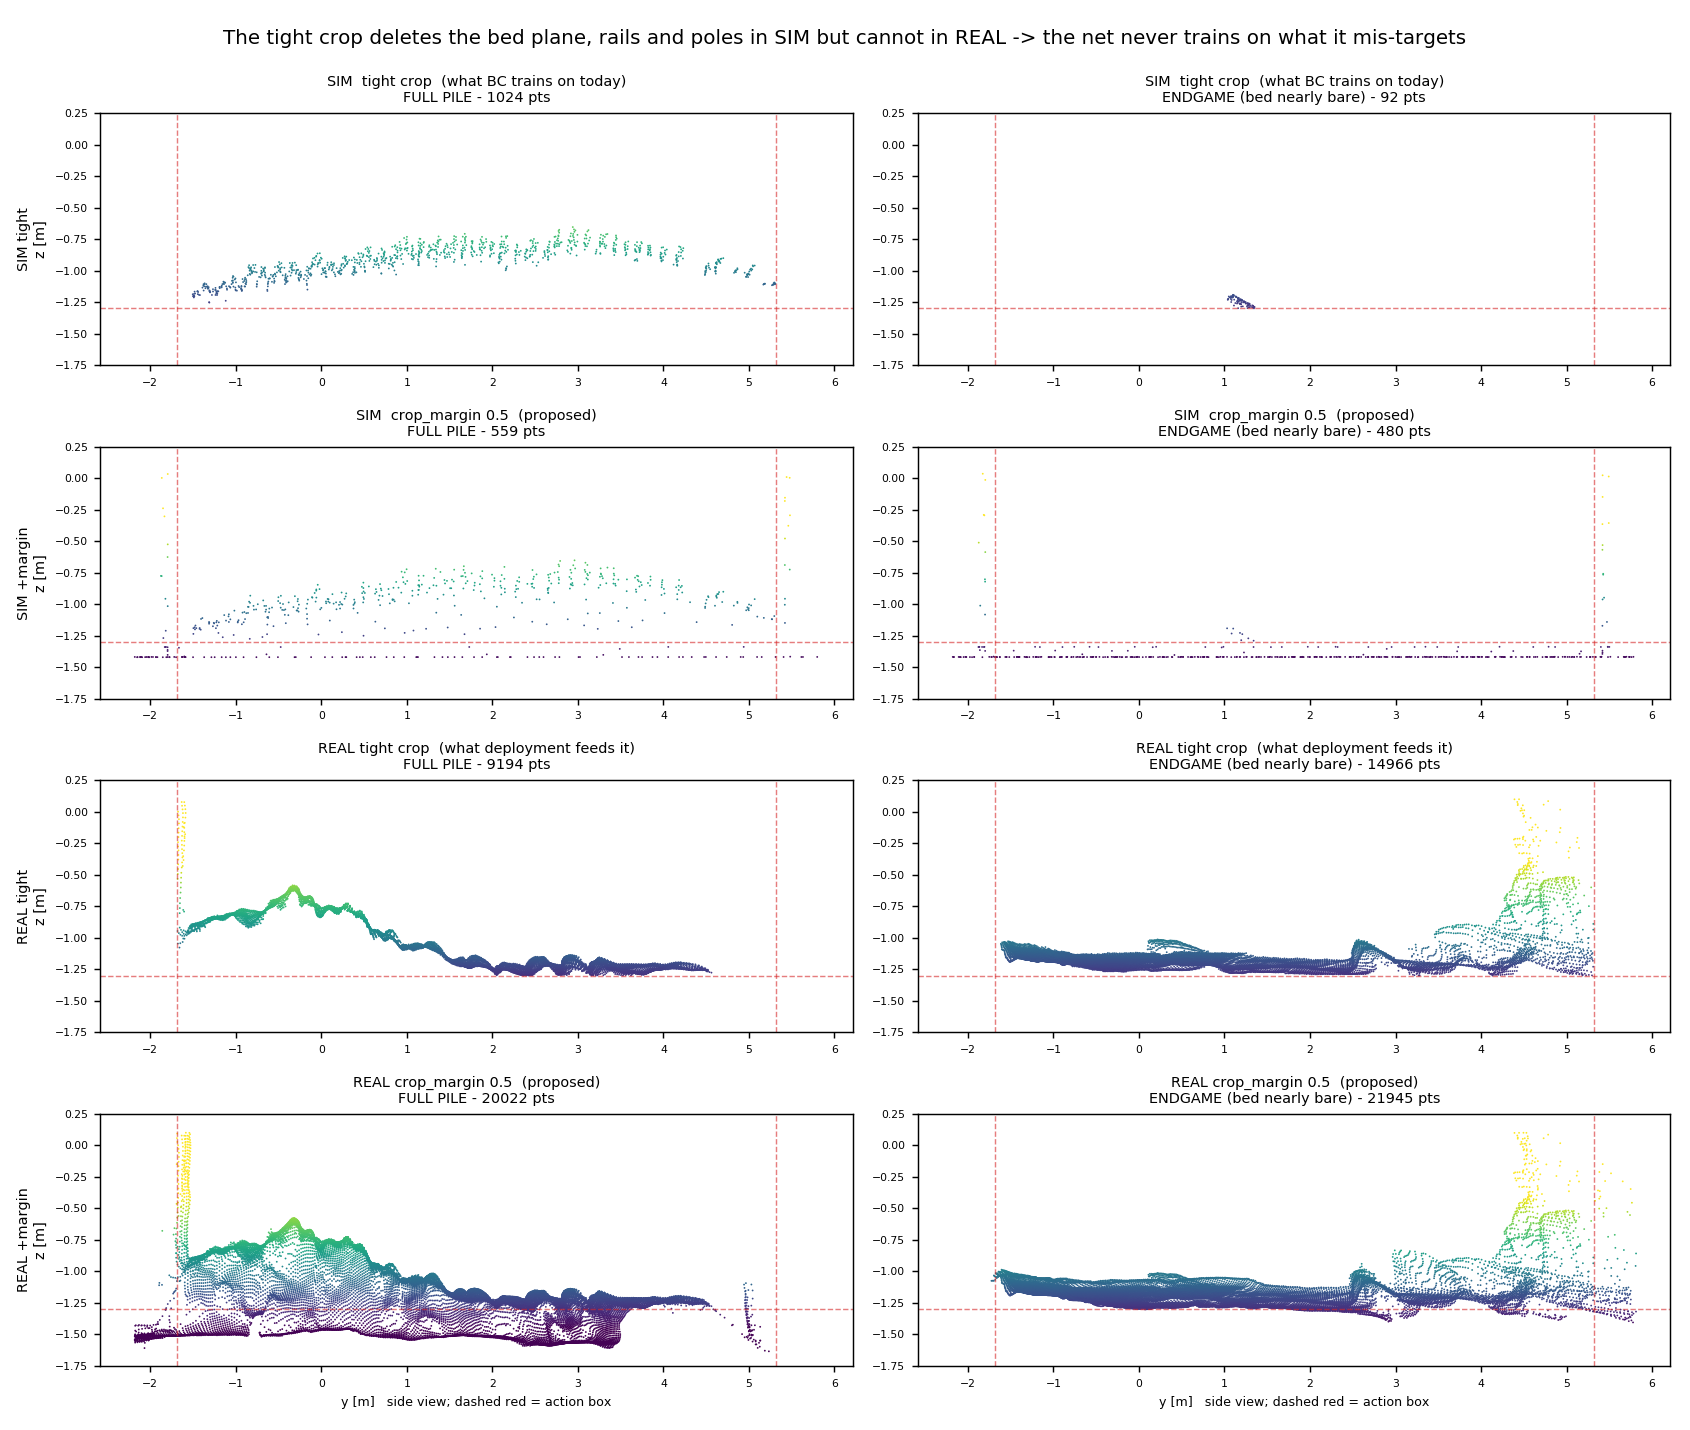
\includegraphics[width=\linewidth]{figures/sim_vs_real_crop.png}
\caption{Side views ($y$--$z$) of simulated and real clouds under the tight
crop and the widened ($m = 0.5$~m) crop, for a full pile (left column) and a
late-trial state (right column); dashed red lines mark the action box. The
tight crop deletes the bed plane, rails, and poles in simulation but cannot
do so on the real crane, where they dominate the late-trial cloud. The
margin crop makes the training observation contain the same structure classes
as the deployment observation.}
\label{fig:bc_sim_vs_real_crop}
\end{figure}

\subsection{Sensor noise model}
\label{sec:bc_noise}

Clouds are collected clean and corrupted with fresh noise at every training
epoch, using an axial noise model fitted to the real ZED stereo camera. Each
point is displaced along its camera ray with a standard deviation that grows
quadratically with range:
\begin{equation}
  \tilde{p}_i = p_i + \eta_i \, \frac{p_i - c}{\lVert p_i - c \rVert}, \qquad
  \eta_i \sim \mathcal{N}\!\left(0,\; \sigma^2(r_i)\right), \qquad
  \sigma(r_i) = \nu \, r_i^2,
\end{equation}
where $c$ is the camera position in the base frame (stored with each dataset),
$r_i = \lVert p_i - c \rVert$, and $\nu = 0.0014$~m$^{-1}$. Padded slots
are left untouched. Applying the noise per epoch rather than at collection
time means every pass over the data sees a different corruption, which
regularizes both policies at no additional collection cost.

\section{The Regression Policy}
\label{sec:bc_regression}

\subsection{Action parameterization}
\label{sec:bc_action_param}

The regression policy outputs a five-dimensional action
$a = (a_x, a_y, a_z, a_c, a_s)$ that encodes the grasp center and yaw. The
three position components are encoded by normalizing the metric target to the
action box and applying the inverse hyperbolic tangent,
\begin{equation}
  u_j = \mathrm{clip}\!\left( \frac{2\,(t_j - b^{\min}_j)}{b^{\max}_j - b^{\min}_j} - 1,\;
        -0.999,\; 0.999 \right), \qquad
  a_j = \operatorname{artanh}(u_j), \qquad j \in \{x, y, z\},
  \label{eq:arctanh_enc}
\end{equation}
so that at deployment the unbounded network output decodes to a target that is
guaranteed to lie inside the box:
\begin{equation}
  \hat{t}_j = b^{\min}_j + \frac{\tanh(\hat{a}_j) + 1}{2}
              \left( b^{\max}_j - b^{\min}_j \right).
  \label{eq:arctanh_dec}
\end{equation}

Yaw is encoded as the cosine and sine of the \emph{doubled} angle,
\begin{equation}
  a_c = \cos 2\psi, \qquad a_s = \sin 2\psi, \qquad
  \hat{\psi} = \tfrac{1}{2} \operatorname{atan2}(\hat{a}_s, \hat{a}_c).
  \label{eq:yaw_enc}
\end{equation}
Doubling the angle folds the grapple's $\pi$-symmetry into the encoding: a
grasp at yaw $\psi$ and one at $\psi + \pi$ are physically identical, and
under Equation~\eqref{eq:yaw_enc} they map to the same label. This is not a
refinement but a requirement. With yaw encoded as a single scalar the expert
labels are contradictory (the same pile state can carry labels $\psi$ and
$\psi + \pi$), the regression cannot converge, and validation error plateaus
an order of magnitude higher; switching to the doubled cosine/sine encoding on
identical data reduced validation error by roughly a factor of nine.

\subsection{Architecture}

The policy is a PointNet encoder followed by a small fully connected actor
head. The encoder applies a shared per-point multilayer perceptron (MLP) to
every point and pools with a channelwise maximum, which makes the network
invariant to point ordering:
\begin{equation}
  h_i = \phi(p_i) \in \mathbb{R}^{256}, \qquad
  g = \rho\!\left( \max_{i = 1, \dots, N} h_i \right) \in \mathbb{R}^{256},
  \label{eq:pointnet}
\end{equation}
where $\phi$ is the per-point MLP $3 \to 64 \to 128 \to 256$ (linear layers
with batch normalization and ELU activations), the maximum is taken per
channel over all points, and $\rho$ is a linear projection $256 \to 256$ with
batch normalization and ELU. The actor head maps the global feature to the
action through dropout ($p = 0.2$) and an MLP $256 \to 128 \to 64 \to 5$ with
ELU activations:
\begin{equation}
  \hat{a} = \mathrm{MLP}_{\mathrm{actor}}\!\left( \mathrm{drop}(g) \right).
\end{equation}
The head dimensions deliberately match the actor of the reinforcement-learning
policies so that behavior-cloned weights load directly into the actor-critic
used for BC-to-RL fine-tuning.

\subsection{Training objective and optimization}

Training minimizes the mean-squared error between predicted and encoded expert
actions over the dataset:
\begin{equation}
  \mathcal{L}_{\mathrm{reg}}(\theta) =
  \frac{1}{|\mathcal{B}|} \sum_{k \in \mathcal{B}}
  \left\lVert \pi_\theta(P_k) - a_k \right\rVert_2^2 .
  \label{eq:mse}
\end{equation}
The optimizer is AdamW with learning rate $10^{-4}$ and weight decay
$10^{-4}$, batch size 64, gradient-norm clipping at 1.0, an
85\,/\,15 train\,/\,validation split, a reduce-on-plateau schedule (factor
0.5, patience 10 epochs), early stopping after 30 epochs without validation
improvement, and checkpointing of the best-validation-loss weights. The
per-epoch ZED noise of Section~\ref{sec:bc_noise} is applied to every training
batch; validation runs on clean clouds.

\subsection{Digging-depth relabeling and the label-clamping problem}
\label{sec:bc_dig}

The sim expert grasps at the log center, $0.056$~m below the local surface.
Real grapple close mechanics need a deeper bite: executed real grasps sit
$0.2$--$0.4$~m below the surface, and a hardware probe with the sim convention
raked across the pile without closing. The dataset is therefore relabeled to a
deployment digging depth $d$ by exploiting the identity
$t_z = z_{\mathrm{surf}} - r_{\log}$:
\begin{equation}
  t_z' = \max\!\left( t_z + r_{\log} - d,\; z_{\mathrm{floor}} \right),
  \label{eq:dig}
\end{equation}
where $z_{\mathrm{floor}}$ is the platform bed floor plus a safety margin
(the executable envelope). Only the label changes; the expert's executed
trajectories, and hence the collected cloud distribution, are untouched.

The clamp in Equation~\eqref{eq:dig} creates a problem specific to the
regression parameterization. With $d = 0.25$~m a large fraction of labels hit
the floor, so the $z$ label distribution is flattened toward a constant and
the regression target loses much of its dependence on the input; the effect
is visible directly in the relabeled dataset
(Figure~\ref{fig:bc_dataset_samples}), where most grasp labels sit in a
narrow band at the bottom of the action box. For the regression policy this
degrades the entire five-dimensional target jointly, since one loss
supervises all components. The scoring policy is immune to this coupling
because depth is supervised separately from target selection
(Section~\ref{sec:bc_scoring_loss}).

\begin{figure}[t]
\centering
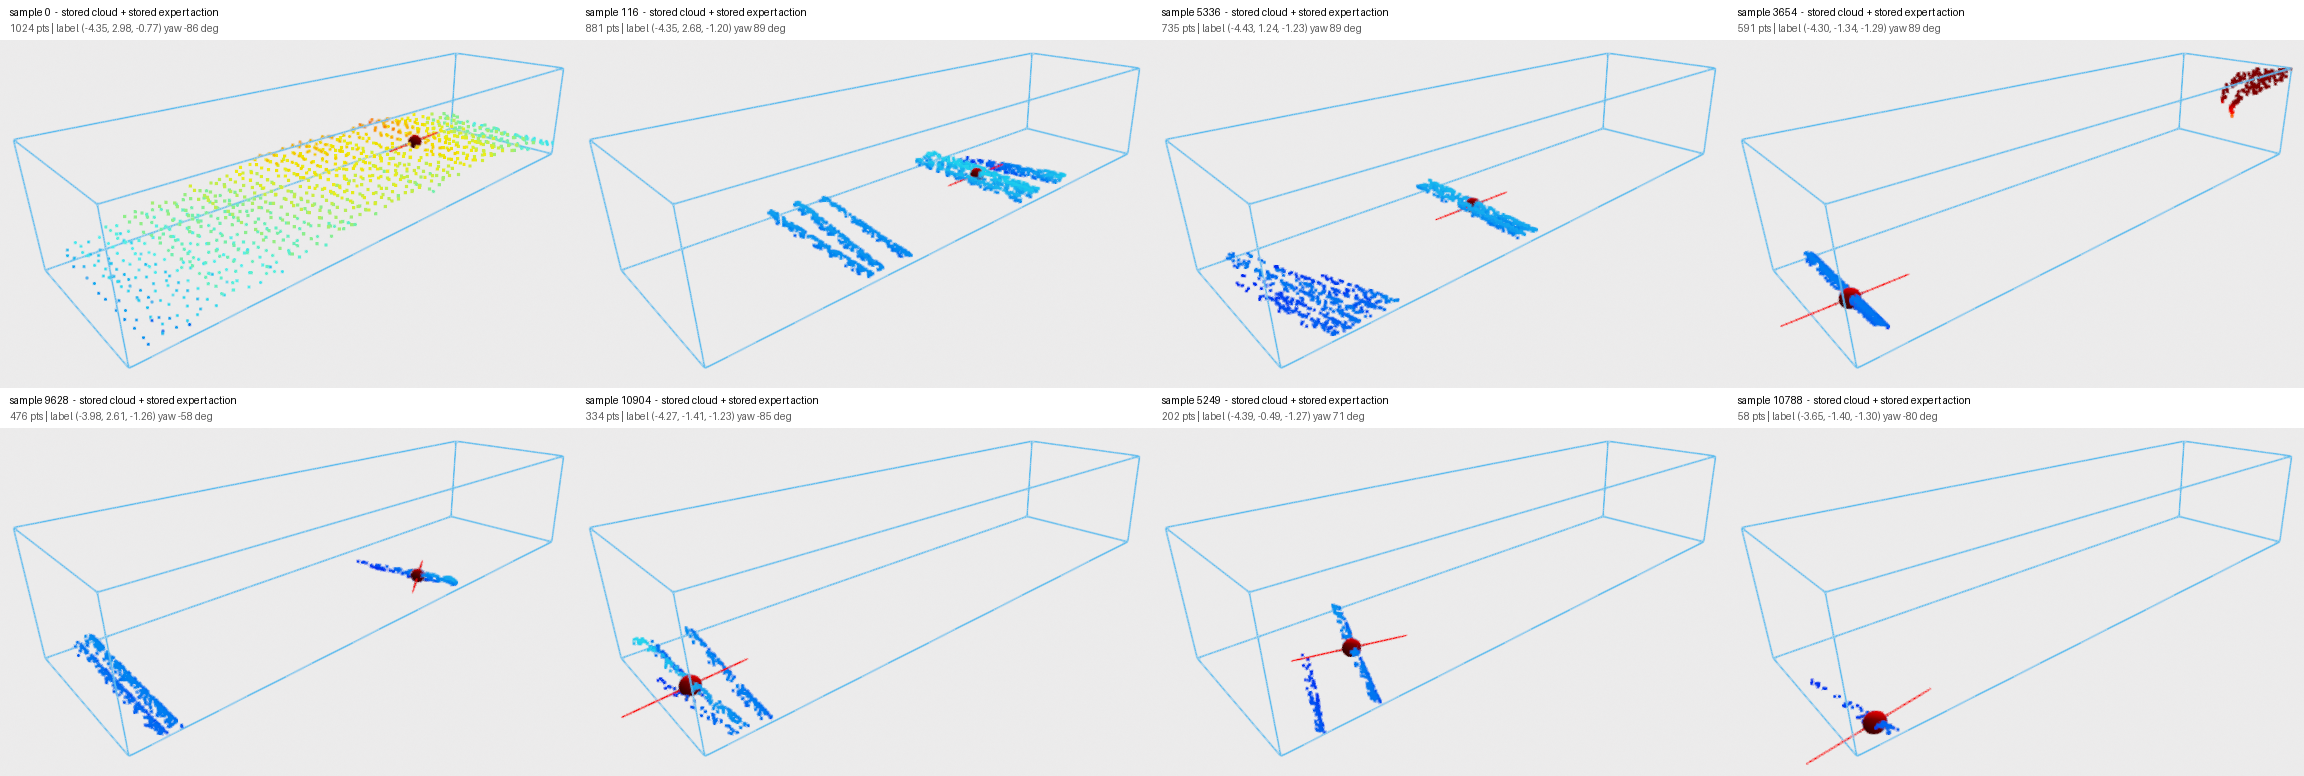
\includegraphics[width=\linewidth]{figures/dataset_samples_aug1v2.png}
\caption{Stored training tuples from a tight-crop dataset after dig
relabeling to $d = 0.25$~m: observed cloud, expert grasp center (sphere), and
commanded yaw (line). The samples span the episode from full pile to
near-empty rack. Most relabeled grasp heights lie in the narrow band at the
bottom of the action box, the flattening that Equation~\eqref{eq:dig}
imposes on the regression $z$ target.}
\label{fig:bc_dataset_samples}
\end{figure}

\subsection{Shape augmentations}

Because early datasets were collected over flat piles, the trainer supports a
family of label-consistent shape augmentations applied per batch in encoded
action space (decode with Equation~\eqref{eq:arctanh_dec}, transform in
meters, re-encode with Equation~\eqref{eq:arctanh_enc}): a vertical shift of
cloud and label by a common $\Delta z \sim \mathcal{U}(0, z_{\max})$ to teach
$z$-equivariance for piles taller than the training distribution, and a mound
warp that reshapes the cloud into a profile peaked at the label position to
teach peak-targeting. With the profiled-pile collection these are no longer
the primary source of shape diversity but remain available. All
augmentations leave zero-padded slots untouched.

\section{The Scoring Policy}
\label{sec:bc_scoring}

\subsection{Motivation: mode averaging under a regression loss}
\label{sec:bc_mode_avg}

The minimizer of the mean-squared error in Equation~\eqref{eq:mse} is the
conditional mean of the label given the observation,
\begin{equation}
  \pi^*(P) = \mathbb{E}\left[ a \mid P \right].
\end{equation}
When the expert's behavior is unimodal this is the right answer. On a pile
with two near-equal mounds it is not: the expert grasps one mound or the
other depending on millimeter-scale height differences, so conditioned on the
observable cloud the label distribution is bimodal, and its mean lies in the
empty gap between the mounds. The policy then commands a grasp over air.

This failure was measured directly. On procedurally generated near-tie
two-mound scenes, the privileged expert and the geometric heuristic (both of
which select a candidate by argmax) aim into the gap in $0\%$ of scenes,
while the regression policy aims into the gap in $33.9\%$ of scenes (and in
$21\%$ of those the commanded grasp closes on nothing); an RL-fine-tuned
regression policy reached $48.5\%$. On the real crane the failure is
absorbing: a grasp over a gap disturbs nothing, so the next observation is
identical and the deterministic policy re-issues the same target, which was
observed for five consecutive cycles in a field trial
(Section~\ref{sec:bc_trials}). In simulation the same
failure costs about three extra cycles per pile, because failed grasps still
nudge logs and eventually let the policy escape.

The scoring policy removes this failure by construction: instead of
regressing coordinates, it classifies \emph{which observed point} to grasp.
A classification loss cannot be minimized by averaging two modes, and an
argmax over observed points cannot select empty space.

\subsection{Architecture}

The scoring policy reuses the PointNet trunk of
Equation~\eqref{eq:pointnet} with identical layer sizes, with one change: the
per-point features $h_i$, which the regression encoder discards at the
max-pool, are returned alongside the pooled global feature $g$. Encoder
weights therefore remain load-compatible between the two policies, and the
frozen-encoder BC-to-RL recipe carries over unchanged.

A shared per-point head conditions each point on the global context. For
every point $i$ the head consumes the concatenation of its per-point feature,
the global feature (after dropout, $p = 0.2$), and its raw coordinates,
\begin{equation}
  e_i = \mathrm{MLP}_{\mathrm{head}}\!\left( \left[ h_i;\, \mathrm{drop}(g);\, p_i \right] \right)
  \in \mathbb{R}^{64},
\end{equation}
with $\mathrm{MLP}_{\mathrm{head}}: 515 \to 128 \to 64$ (ELU activations),
and three linear output heads read off
\begin{equation}
  s_i = w_s^\top e_i \in \mathbb{R}, \qquad
  \delta_i = w_\delta^\top e_i \in \mathbb{R}, \qquad
  q_i = W_q\, e_i \in \mathbb{R}^2,
\end{equation}
a grasp-quality logit $s_i$, a vertical residual $\delta_i$ from the point to
the commanded grasp center, and a per-point yaw $q_i = (q_i^c, q_i^s)$ in the
doubled-angle encoding of Equation~\eqref{eq:yaw_enc}. Padded slots receive
$s_i = -\infty$ so they can never win the argmax. The horizontal coordinates
$x$ and $y$ are not predicted: they are read off the selected point. Depth is predicted
only as a residual from the selected surface point, not as an absolute
coordinate.

\subsection{Label construction and training objective}
\label{sec:bc_scoring_loss}

The scoring policy trains on the same datasets as the regression policy; no
recollection is needed. Stored regression labels are decoded back to metric
targets $(t, \psi)$ with Equations~\eqref{eq:arctanh_dec} and
\eqref{eq:yaw_enc}, and the classification target becomes the observed
(non-padded) point nearest the expert grasp in the horizontal plane:
\begin{equation}
  i^* = \operatorname*{arg\,min}_{i}\; d^{\mathrm{xy}}_i, \qquad
  d^{\mathrm{xy}}_i = \left\lVert p_{i,xy} - t_{xy} \right\rVert_2 .
\end{equation}
Because FPS-sampled neighbors of $i^*$ are often near-identical grasp
candidates, the hard label is smoothed over a horizontal radius
$\rho = 0.12$~m: the target distribution $y$ is uniform over
$\{ i : d^{\mathrm{xy}}_i \le \rho \} \cup \{ i^* \}$ and zero elsewhere. The radius is
smaller than any physical gap between mounds, so smoothing shares probability
among interchangeable neighbors without ever bridging the gap whose avoidance
motivates the classification loss in the first place.

The loss combines cross-entropy on the scores with regression terms evaluated
\emph{only at the labeled point}:
\begin{align}
  \mathcal{L}_{\mathrm{cls}} &= - \sum_{i=1}^{N} y_i \,
      \log \operatorname{softmax}(s)_i, \\
  \mathcal{L}_{\delta} &= \left( \delta_{i^*} - \left( t_z - p_{i^*, z} \right) \right)^2, \qquad
  \mathcal{L}_{\mathrm{yaw}} = \left\lVert q_{i^*} -
      \left( \cos 2\psi,\, \sin 2\psi \right) \right\rVert_2^2, \\
  \mathcal{L}_{\mathrm{score}} &= \mathcal{L}_{\mathrm{cls}}
      + \lambda_\delta \, \mathcal{L}_{\delta}
      + \lambda_{\mathrm{yaw}} \, \mathcal{L}_{\mathrm{yaw}},
  \qquad \lambda_\delta = 1.0, \quad \lambda_{\mathrm{yaw}} = 0.5 .
  \label{eq:scoring_loss}
\end{align}
No per-point annotation is required. The dataset holds one expert grasp per
cloud, the same $(P_k, t_k, \psi_k)$ tuples the regression policy consumes,
and the per-point targets are derived from that grasp at training time.
Three properties follow. First, the scores are not regressed toward
prescribed values: cross-entropy constrains only the softmax-normalized
ranking, so raising the labeled point's score lowers every other point's
normalized probability and the $N - 1$ unlabeled points receive implicit
downward pressure. The head therefore learns a relative log-odds that the
expert would grasp at a point, invariant to a constant offset across the
cloud, which is the quantity the argmax requires. The structure negatives of
Section~\ref{sec:bc_scoring_aug} are the only supervision that lowers
individual scores explicitly. Second, the depth and yaw heads receive
gradient at the labeled point only; their outputs at the remaining points
are unconstrained by Equation~\eqref{eq:scoring_loss} and generalize through
the shared per-point head, which is what makes them usable at whichever
point wins the argmax. Third, the horizontal coordinates are not predicted,
so they require no supervision.

Optimization mirrors the regression policy: AdamW with learning rate
$10^{-4}$ and weight decay $10^{-4}$, batch size 64, an 85\,/\,15 split, a
reduce-on-plateau schedule, per-epoch ZED noise, and best-validation
checkpointing. Alongside the validation loss, training reports the median
horizontal error of the decoded grasp and the fraction of validation scenes
within $0.30$~m of the expert target.

The digging-depth convention of Equation~\eqref{eq:dig} is applied to the
metric label $t_z$ before computing the residual target
$t_z - p_{i^*, z}$. It therefore shifts only the depth head; the
classification target, which point to grasp, is untouched, so the
label-clamping problem of Section~\ref{sec:bc_dig} cannot collapse the
selection signal.

The residual target is close to constant over much of the dataset, which
follows from its construction. Where the clamp in Equation~\eqref{eq:dig} is
inactive and the selected point lies on the same local surface as the label,
$t_z - p_{i^*, z} = -d$ exactly. On the margin dataset used for the deployed
checkpoint ($d = 0.25$~m, floor at $-1.20$~m) the labeled point sits a median
of $0.041$~m from the expert target in the horizontal plane, and the residual
targets have mean $-0.125$~m with standard deviation $0.144$~m. The two
regimes behave differently. On the $42\%$ of samples where the clamp is
inactive the residual is grouped near $-d$ (mean $-0.207$~m, standard
deviation $0.112$~m), the remaining spread coming from log curvature and from
the sampled point not coinciding with the surface height at the label. On the
$58\%$ where the label is pinned to the floor the residual becomes
$z_{\mathrm{floor}} - p_{i^*, z}$ and therefore varies directly with the
height of the selected point (mean $-0.062$~m, standard deviation
$0.134$~m), turning positive where that point lies below the floor plane. The
head thus predicts a near-constant bite depth in the free regime and a
floor-referenced correction in the clamped one. In both regimes the commanded
height is anchored to the selected point rather than to the global frame,
which is the property that makes the parameterization insensitive to pile
height.

\subsection{Inference}

At deployment the grasp is decoded from the highest-scoring admissible point
(Algorithm~\ref{alg:scoring_decode}):
\begin{equation}
  \hat{i} = \operatorname*{arg\,max}_{i \,\in\, \mathcal{C}} s_i, \qquad
  \hat{t} = \left( p_{\hat{i},x},\; p_{\hat{i},y},\; p_{\hat{i},z} + \delta_{\hat{i}} \right), \qquad
  \hat{\psi} = \tfrac{1}{2} \operatorname{atan2}\!\left( q_{\hat{i}}^s,\, q_{\hat{i}}^c \right).
\end{equation}
The \emph{candidate mask} defines the admissible set: $\mathcal{C}$ contains
the non-padded points that lie inside the action box
$[b^{\min}, b^{\max}]$. It is always active, in offline evaluation and in
the deployed node alike, where the box is supplied as a runtime parameter and
set to the same training-coordinate action box the policy was trained
against. The mask is required by the widened observation crop: with
$m > 0$ the input cloud deliberately contains points outside the action box
(bed apron, rack posts and rails, pole bases in the margin band). Those
points are observation \emph{context}, and the network is free to use them to
judge the scene, but they are not commandable grasps, so selecting one would
issue an unreachable or unsafe target. Without the mask, an argmax on a real
cloud selected a margin-band point beside tall structure, outside the
reachable volume. Masking is applied to the
score before the argmax, so a masked point can never win regardless of its
score, and the same rule carries over unchanged to reinforcement learning,
where it becomes exact logit masking in the action distribution.

A second, \emph{optional} filter exists but was not used in any result
reported here. The \emph{support gate} further restricts $\mathcal{C}$ to
points whose local horizontal neighborhood is well populated: with
$n_i = \left| \{ j : \lVert p_{j,xy} - p_{i,xy} \rVert < r_s \} \right|$ and
$r_s = 0.5$~m, a point survives only if $n_i \ge \kappa \max_j n_j$. It was
introduced because a raw argmax can in principle be won by a single
noise-displaced point, a failure characterized in simulation on the
tight-crop policy (Section~\ref{sec:bc_noise_sweep}). The margin-trained
policy did not exhibit that failure, so the gate is disabled by default and
was disabled in both hardware trials and in every number quoted in this
chapter; it is retained only as an opt-in safeguard for the tight-crop
checkpoint. Because it is pure geometric post-processing rather than
learning, keeping it off means the results credit the learned
discrimination alone.

\begin{algorithm}[t]
\caption{Scoring-policy inference with admissibility masking}
\label{alg:scoring_decode}
\begin{algorithmic}
\algin{Observation cloud $P$ with padding mask
(Algorithm~\ref{alg:obs_pipeline}); trained scoring network; action box
$[b^{\min}, b^{\max}]$; support-gate flag (disabled by default).}
\algout{Grasp target $\mathbf{g} = (\hat{t}_x, \hat{t}_y, \hat{t}_z, \hat{\psi})$.}

\algstage{1.\;Forward pass}
\State $\{h_i\}, g \gets \mathrm{PointNet}(P)$
\Comment{per-point features and the pooled global feature}
\State $e_i \gets \mathrm{MLP}_{\mathrm{head}}\big([\,h_i;\, g;\, p_i\,]\big)$ for all $i$
\State $s_i \gets w_s^\top e_i$, \quad
       $\delta_i \gets w_\delta^\top e_i$, \quad
       $q_i \gets W_q e_i$

\algstage{2.\;Admissibility mask}
\State $\mathcal{C} \gets \{\, i : p_i \text{ is not padding and } b^{\min} \preceq p_i \preceq b^{\max} \,\}$
\If{support gate enabled}
  \State $n_i \gets \big| \{ j : \lVert p_{j,xy} - p_{i,xy} \rVert < r_s \} \big|$
  \State $\mathcal{C} \gets \{\, i \in \mathcal{C} : n_i \ge \kappa \max_j n_j \,\}$
  \Comment{off in every result reported here}
\EndIf
\State $s_i \gets -\infty$ for all $i \notin \mathcal{C}$
\Comment{applied to the score, so a masked point can never win}

\algstage{3.\;Decode}
\State $\hat{\imath} \gets \operatorname*{arg\,max}_{i} s_i$
\State $(\hat{t}_x, \hat{t}_y) \gets (p_{\hat{\imath},x},\, p_{\hat{\imath},y})$
\Comment{read off the point, not predicted}
\State $\hat{t}_z \gets p_{\hat{\imath},z} + \delta_{\hat{\imath}}$
\Comment{residual from the selected surface point}
\State $\hat{\psi} \gets \tfrac{1}{2}\operatorname{atan2}(q^s_{\hat{\imath}},\, q^c_{\hat{\imath}})$
\State Clamp $\hat{t}_z$ to the bed-floor envelope (Section~\ref{sec:s2r_deploy})
\State \Return $(\hat{t}_x, \hat{t}_y, \hat{t}_z, \hat{\psi})$
\end{algorithmic}
\end{algorithm}

\subsection{Augmentations specific to the scoring parameterization}
\label{sec:bc_scoring_aug}

Two augmentations exploit or extend the classification structure.

\emph{Rigid horizontal shift.} The cloud and the label are translated by a
common offset drawn uniformly from $[-v, v]$ per axis in $x$ and $y$, with
padded slots left at the origin; the deployed checkpoint used
$v_x = 0.15$~m and $v_y = 0.5$~m. Because the classification label is a
point index, the translation maps the label to itself and no relabeling is
needed, so the augmentation supplies additional samples at no supervision
cost. The same augmentation applied to a regression policy changes the
numeric target and requires it to fit its coordinate map over the enlarged
domain (Section~\ref{sec:bc_differences}). Note that both policies are still
deployed against a calibrated crop box; the augmentation widens the range of
scene positions seen in training, it does not remove the need for
calibration. The vertical axis is not
augmented, because the bed floor and gravity are physical rather than
calibration choices.

\emph{Structure negatives.} The collected margin clouds contain full-height
pole columns, whereas the real rack also presents broken poles cut down to
short stubs. A pole-variation augmentation supplies the missing heights from
the columns already in the data, without recollection and without inserting
synthetic geometry. Pole-like columns are detected once per cloud as
clusters of points reaching above the pile ceiling. Each epoch, with
probability $0.7$ a cloud is varied at all; within a varied cloud each column
draws $u \sim \mathcal{U}(0,1)$ and is kept intact for $u < 0.25$, cut to a
stub of height $\mathcal{U}(0.08, 0.6)$~m for $0.25 \le u \le 0.90$, and cut
nearly flush at $0.05$~m for $u > 0.90$. Points above the cut are removed and
the point count is held fixed by zero padding, so the tensor shape is
unchanged. Cross-entropy alone gives a known-structure point no more downward
pressure than any other non-label point, so the pole points that survive the
draw are additionally driven negative with a softplus penalty on their raw
scores:
\begin{equation}
  \mathcal{L}_{\mathrm{neg}} = \frac{1}{|\mathcal{S}|} \sum_{i \in \mathcal{S}}
  \log\!\left( 1 + e^{s_i} \right),
\end{equation}
added to Equation~\eqref{eq:scoring_loss} with weight $w_{\mathrm{neg}}$,
where $\mathcal{S}$ is the set of pole points surviving the draw
(Figure~\ref{fig:bc_stub_aug}). The scoring policy deployed in the hardware
trials of Section~\ref{sec:bc_trials} was trained with this augmentation and
with the explicit negatives.

\begin{figure}[t]
\centering
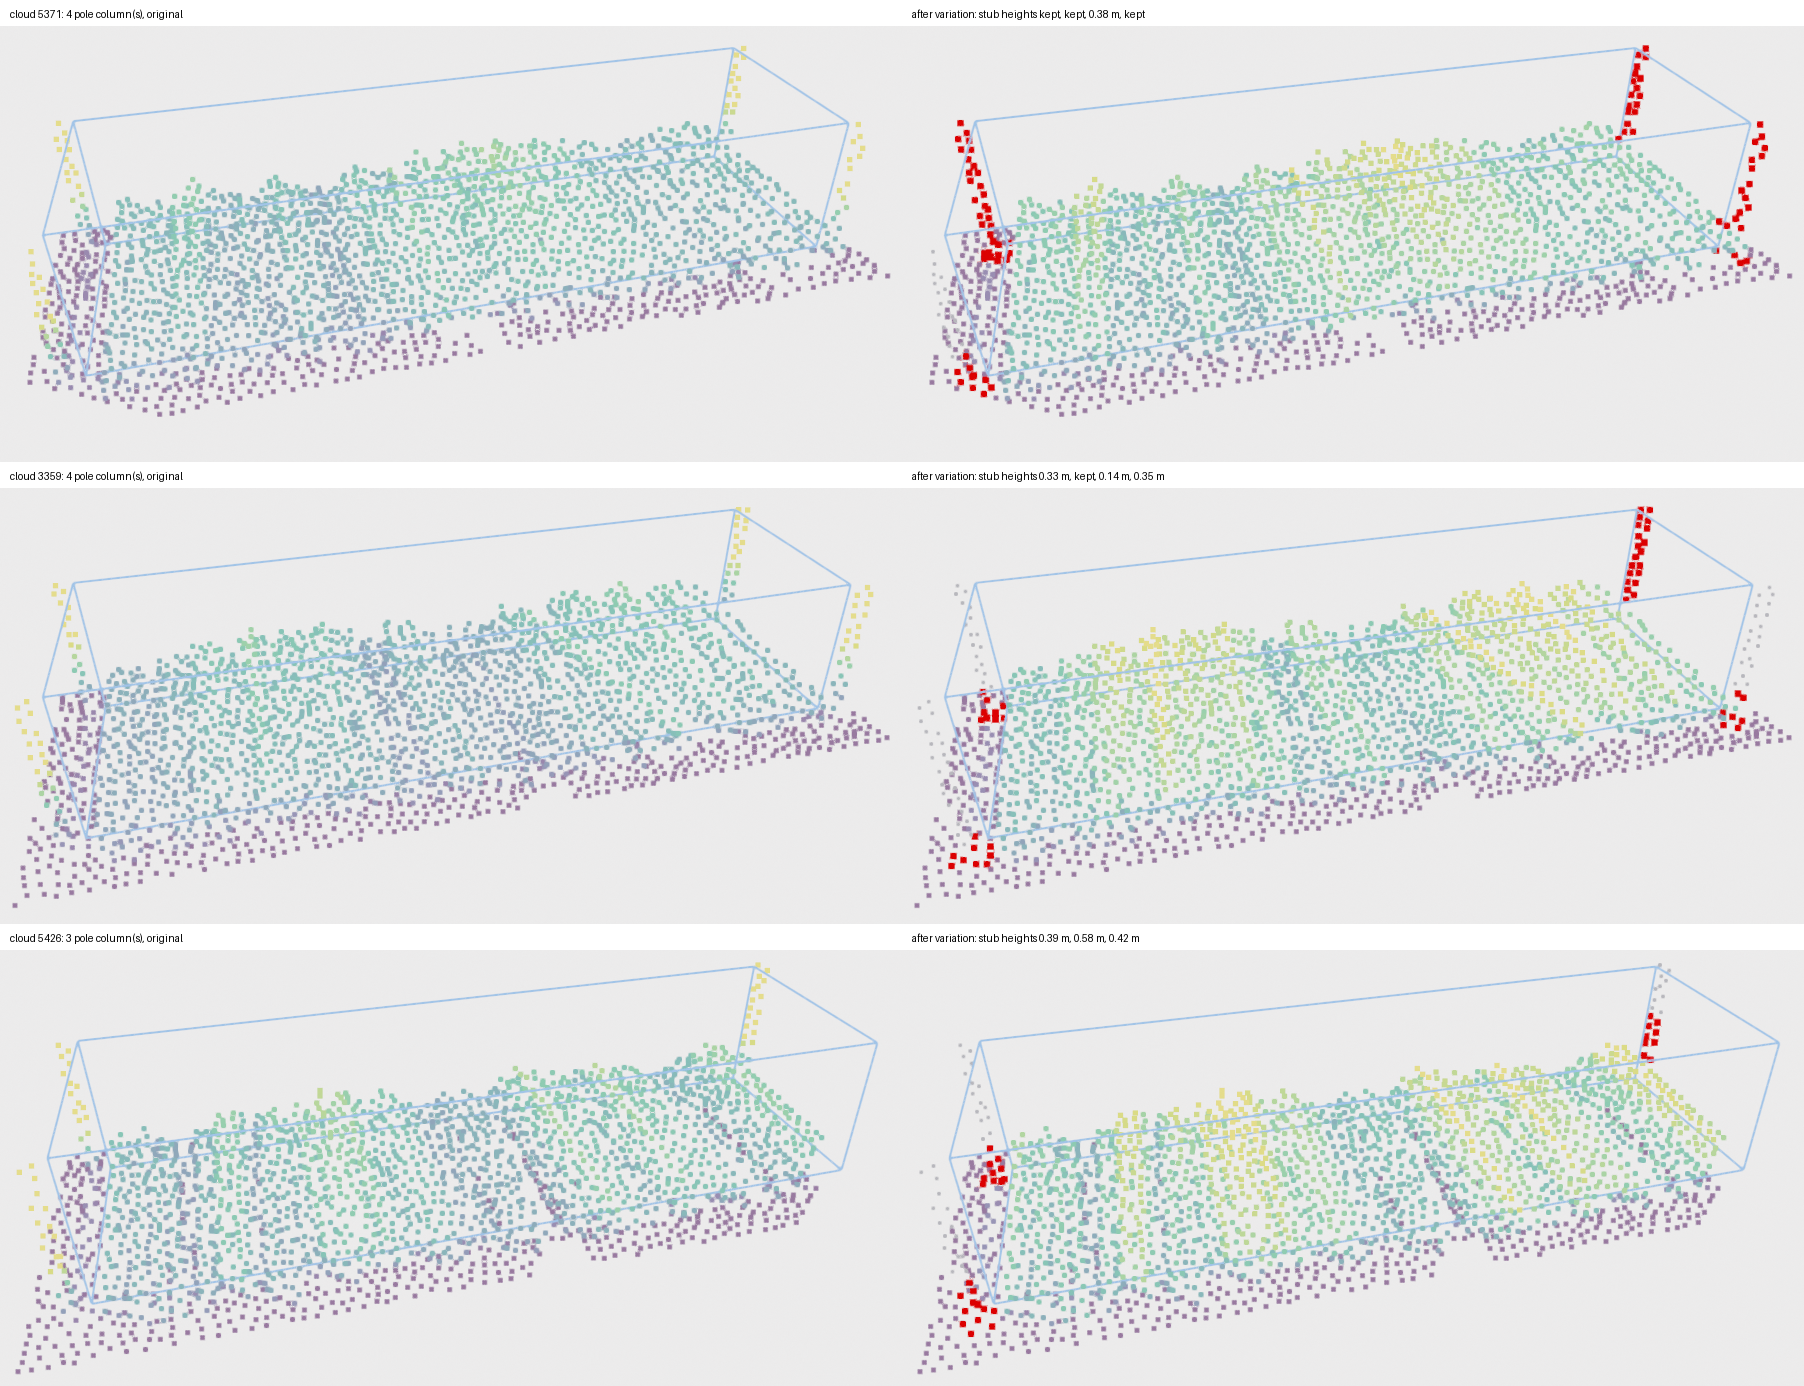
\includegraphics[width=\linewidth]{figures/pole_variation.png}
\caption{Pole-variation augmentation on three margin-dataset clouds (rows).
Left: the collected cloud, with full-height pole columns at the corners of
the crop. Right: one draw of the augmentation, with removed points shown as
grey ghosts at their original positions and the surviving pole points, which
form the negative set $\mathcal{S}$, in red. Realized stub heights are given
per column above each panel; columns drawn as kept retain their full height
and still contribute negatives.}
\label{fig:bc_stub_aug}
\end{figure}

\section{Explicit Differences}
\label{sec:bc_differences}

Table~\ref{tab:bc_differences} summarizes the two policies. Everything
upstream is shared: the same expert, the same datasets, the same cloud
preprocessing, the same noise model, the same PointNet trunk with
load-compatible weights, and the same optimizer settings. The policies differ
in five places, each a consequence of the output parameterization.

\begin{table}[t]
\centering
\caption{Regression versus scoring BC policies. Shared components: expert
demonstrations, datasets, cloud preprocessing, ZED noise augmentation,
PointNet trunk (per-point MLP $3 \to 64 \to 128 \to 256$, max-pool, projection
to $256$), AdamW ($10^{-4}$, weight decay $10^{-4}$), batch size 64,
85\,/\,15 split, plateau schedule, best-validation checkpointing.}
\label{tab:bc_differences}
\begin{tabular}{p{0.24\linewidth} p{0.34\linewidth} p{0.34\linewidth}}
\hline
 & \textbf{Regression} & \textbf{Scoring} \\
\hline
Output & One global 5D vector: box-normalized $\operatorname{artanh}$ $(x,y,z)$, $(\cos 2\psi, \sin 2\psi)$ & Per-point logit $s_i$, depth residual $\delta_i$, yaw $q_i$; grasp read off the argmax point \\
Features used & Global max-pooled feature only & Per-point features and global feature \\
Loss & MSE on the 5D vector, Eq.~\eqref{eq:mse} & Cross-entropy over points + MSE at the labeled point, Eq.~\eqref{eq:scoring_loss} \\
Optimal predictor & Conditional mean of the expert action & Conditional mode over observed points \\
Multimodal scenes & Averages modes; can aim into the gap between mounds & Commits to one mound; target always on observed material \\
Depth & Absolute $z$ in the action box & Residual from the selected surface point \\
Dig relabeling & Floor clamp flattens $z$ labels; couples into the joint loss & Affects the residual head only; selection signal untouched \\
Translation & Coordinates are learned; an uncorrected frame shift displaces the command & Label is an index; rigid-shift augmentation needs no relabeling, and $x, y$ are read off a point rather than extrapolated \\
Inference & Decode, Eq.~\eqref{eq:arctanh_dec}; no masking needed & Candidate mask to the action box (always on); support gate available but unused \\
\hline
\end{tabular}
\end{table}

\subsection{Estimator: mean versus mode}

This is the root difference; the rest follow from it. The regression loss is
minimized by the conditional mean of the expert action, the scoring loss by
the conditional mode over observed points
(Section~\ref{sec:bc_mode_avg}). On unimodal scenes the two agree, and the
policies behave near-identically. On multimodal scenes the mean falls between
modes while the mode commits to one. Replayed on the 26 clouds from the field
trial in which the regression policy locked onto the gap between two mounds,
the scoring policy committed to a mound on 26 of 26 clouds with zero
zero-support targets, against a $27\%$ zero-support rate for the regression
policy on the same clouds. The prediction also held on hardware: on the
double-mound shape where the deployed regression policy executed 15 gap
shots in 26 cycles, the deployed scoring policy produced zero gap-targeting
cycles in 30 (Section~\ref{sec:bc_scoring_trials}).

\subsection{Output space: coordinates versus observed points}

The regression policy can output any point in the action box, including empty
space; the scoring policy can only output observed material (plus a small
learned depth residual). This makes the gap-targeting failure impossible
rather than merely unlikely, but introduces an admissibility concern the
regression policy never has: since any observed point could in principle win,
padded and out-of-box points must be excluded explicitly, which is the
candidate mask. The regression policy needs no equivalent because its
$\tanh$ decode confines its output to the action box by construction. In
effect the regression policy's failure mode is averaging, and the scoring
policy's residual failure mode is trusting a single bad candidate; the
candidate mask closes the reachability half of that, and the optional support
gate exists for the noise half, though the deployed policy did not need it.

\subsection{Depth: absolute versus residual}

Regressing absolute $z$ ties the depth prediction to the global frame and to
the label distribution, which the dig-relabeling clamp then flattens
(Section~\ref{sec:bc_dig}). Predicting a residual from the selected surface
point makes depth local: the network learns "how far below this surface to
bite," which transfers across pile heights and is unaffected by where the
labels sit relative to the floor. The residual parameterization also
sidesteps the $z$-saturation seen when real piles were taller than any sim
training pile, a failure that previously required a dedicated
$z$-shift augmentation for the regression policy.

\subsection{Frame sensitivity}

Neither network is translation invariant: both consume raw coordinates, and
the scoring head concatenates $p_i$ to its per-point input. The difference
lies in what a rigid horizontal shift does to the label and to the output.

For the regression policy the shift changes the label, since the target is a
metric coordinate. The practical consequence appeared when the rack was found
to sit about $0.45$~m in $y$ from the position at which the crop box had been
calibrated. Correcting this is ordinary recalibration, not a policy
mechanism: the offset is measured once and applied as a parameter that
translates the crop box onto the rack, returns the cropped cloud to the
coordinates the network was trained in, and adds the offset back to the
decoded command. What the episode measured is the sensitivity itself. Moving
the crop box by the rack offset without returning the cloud to training
coordinates displaced the regression policy's commanded target by $1.2$ to
$1.6$~m, several times the physical displacement, which shows how tightly a
regressed coordinate is bound to the frame it was trained in.

For the scoring policy the shift leaves the label unchanged, because the
label is a point index rather than a coordinate: translating cloud and label
together maps $i^*$ to itself. The augmentation is therefore label preserving
and generated at no cost, and the deployed checkpoint was trained with
offsets drawn uniformly from $\pm 0.15$~m in $x$ and $\pm 0.5$~m in $y$. The
second effect is on the output path. The horizontal command is read from the
selected point instead of extrapolated from a learned coordinate map, so a
shift can only act through the ranking, and a ranking error that moves the
argmax to a neighboring point on the same material still yields a target on
material. This bounds the failure rather than removing it. The score function
remains shift sensitive through $p_i$, the depth residual and yaw are not
protected by the index argument, and the hardware trials of
Section~\ref{sec:bc_scoring_trials} still ran with the measured rack offset
applied, so
this is a property of the parameterization and not a measured deployment
result.

\subsection{Architecture and BC-to-RL compatibility}

The trunks are identical up to the max-pool, and layer names are
load-compatible; the scoring policy simply keeps the per-point features that
the regression encoder discards. Head capacity differs modestly: the
regression head is an MLP on the global feature, while the scoring head is a
shared per-point MLP on a $515$-dimensional input (per-point feature, global
feature, raw coordinates) with three linear outputs. Because the encoder is
shared and unchanged, the frozen-encoder BC-to-RL fine-tuning recipe
developed for the regression policy applies to the scoring policy without
modification.

\section{Field Trials and Analysis}
\label{sec:bc_trials}

This section reports the hardware evidence: a baseline campaign with the
deployed geometric heuristic whose failure analysis fixed the priorities for
the scoring design, offline replays of both learned policies on the recorded
clouds from those trials, a simulated observation-degradation sweep, and two
hardware trials of the scoring policy. Throughout, a \emph{cycle} is one
grasp-transport-deposit sequence, \emph{success rate} is the fraction of
cycles that deposit at least one log, and \emph{alignment} is an
operator-assigned score from 1 to 5 for how well the grapple met the logs.
Deposition in every trial follows the bin-fill procedure of
Section~\ref{sec:s2r_deposit}.

\subsection{Baseline campaign and failure taxonomy}
\label{sec:bc_baseline_trials}

Three trials of the deployed perception heuristic were run on approximately
200-log piles arranged in three shapes: a double mound, a jagged multi-peak
profile, and a single mound (Table~\ref{tab:bc_baseline_trials}). Pooled, the
baseline grasped at least one log on 67\% of 73 cycles. The jagged profile is
the hard geometry, needing roughly twice the cycles of the mound shapes for
the same inventory.

\begin{table}[t]
\centering
\caption{Baseline (geometric heuristic) field trials. Success is the
fraction of cycles depositing at least one log; $c_{95}$ is the cycle at
which 95\% of the eventually-moved logs had been moved; alignment is the
operator score (1--5).}
\label{tab:bc_baseline_trials}
\begin{tabular}{lcccccc}
\hline
\textbf{Trial} & \textbf{Cycles} & \textbf{Logs} & \textbf{Success \%} &
\textbf{Logs/success} & $c_{95}$ & \textbf{Align.} \\
\hline
Double mound & 18 & 196 & 83.3 & 13.1 & 16 & 4.53 \\
Jagged       & 36 & 193 & 55.6 &  9.7 & 32 & 4.65 \\
Single mound & 19 & 175 & 73.7 & 12.5 & 14 & 4.07 \\
\hline
Pooled       & 73 & 564 & 67.1 & 11.5 & -- & 4.45 \\
\hline
\end{tabular}
\end{table}

Of the 24 empty cycles, 16
(67\% of failures, 22\% of \emph{all} cycles) were caused by the heuristic
targeting rack rails, pole columns, or noise points in the air; 4 were chokes
(grasping too deep for the grapple to close); and 4 were yaw or control
faults. Structure and noise targeting is thus the dominant real-world failure
mode, and it concentrates in the endgame: these failures occurred on average
76\% of the way through a trial (median 82\%), with 11 of 16 in the final
30\% of cycles. The mechanism is geometric. Once the pile drops below the
rack rail height, the rails and poles become the highest points in the crop,
and a highest-point heuristic locks onto them. The failure is absorbing:
grasping a rail changes nothing, so the next cloud is identical and the same
target is reissued. The single-mound trial ended in four consecutive rack
grabs and required manual completion; the jagged trial ended in three.

\begin{figure}[t]
\centering
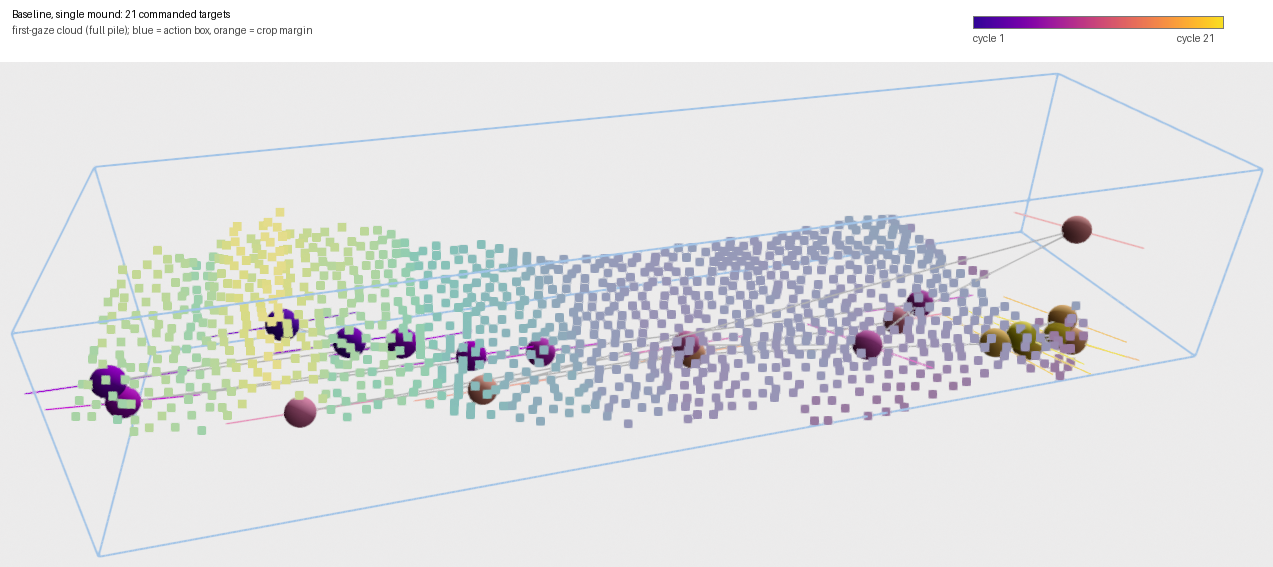
\includegraphics[width=\linewidth]{figures/real_trials/targets_3d_baseline_single.png}
\caption{Every target commanded by the baseline in the single-mound trial,
drawn over the cloud observed at the first cycle. Sphere colour encodes cycle
order, the short line through each sphere is the commanded grapple yaw, and
the blue box is the action volume. Early targets sit on the mound; the final
cycles collapse into a cluster at the far end of the rack, where the end
board and corner poles stand, which is the absorbing lock-in that ended the
trial.}
\label{fig:bc_targets_baseline}
\end{figure}

This taxonomy set the priorities for the scoring policy line: the dominant
failure is a \emph{perception discrimination} failure (log material versus
structure and noise), which is exactly what a learned per-point score can
address, and which motivated the margin crop
(Figure~\ref{fig:bc_sim_vs_real_crop}), the structure negatives
(Section~\ref{sec:bc_scoring_aug}), and the candidate mask.

\subsection{Offline replay on recorded trial clouds}
\label{sec:bc_replay}

Before new hardware time was spent, both policies were replayed offline on
two sets of real clouds: the 26 recorded clouds from the field run in which
the deployed regression policy locked onto the gap between two mounds
(Section~\ref{sec:bc_mode_avg}), and clouds extracted from the baseline
trials' recorded bags, each processed by the pipeline matching the policy
(tight crop at 1024 points, or margin crop at 2048).

On the 26 gap-failure clouds the scoring policy committed to one of the two
mounds on 26 of 26 clouds with zero unsupported targets, against a 27\%
zero-support rate for the regression policy on the same clouds. On the
baseline-trial clouds the qualitative difference is the one predicted by the
estimator argument (Figure~\ref{fig:bc_target_comparison}): the regression
policy places targets at intermediate coordinates between mounds, while the
margin-trained scoring policy selects a point on one mound. The replay also
exposed a genuine weakness of the \emph{tight-crop} scoring variant: on real
clouds it repeatedly selected points on the end board that closes the rack
and on the corner pole columns,
structure it had never observed during training, which is the sim-to-real
asymmetry of Figure~\ref{fig:bc_sim_vs_real_crop} and the reason the
margin-trained variant became the deployment candidate.

\begin{figure}[t]
\centering
\begin{minipage}{0.49\linewidth}
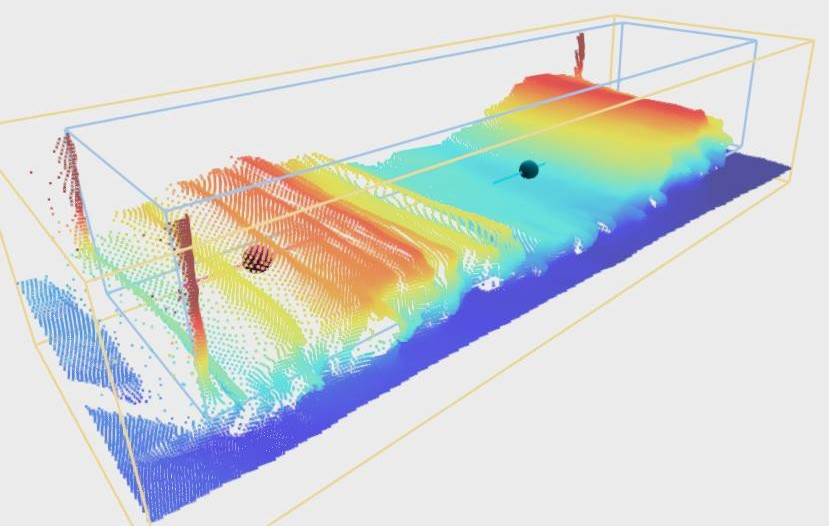
\includegraphics[width=\linewidth]{figures/targets_double_c01.jpg}
\end{minipage}\hfill
\begin{minipage}{0.49\linewidth}
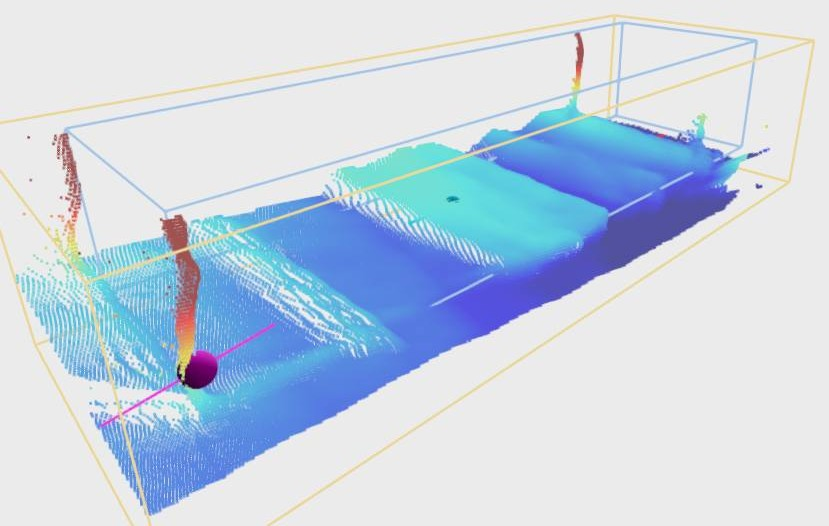
\includegraphics[width=\linewidth]{figures/targets_double_c11.jpg}
\end{minipage}
\caption{Offline policy targets on two recorded double-mound trial clouds
(blue box: action volume; orange box: margin crop; sphere: commanded grasp;
line: commanded yaw). Left: the regression policy (cyan, $y = 2.25$~m) places
its target in the saddle between the two mounds, the conditional-mean
behavior of Section~\ref{sec:bc_mode_avg}, while the margin-trained scoring
policy (red, $y = 3.81$~m) commits to a mound. Right: the tight-crop scoring
variant (magenta) selects a point on a pole column it never saw during
training, while the margin-trained variant, which trains with such structure
in view, targets pile material.}
\label{fig:bc_target_comparison}
\end{figure}

\subsection{Robustness to observation degradation}
\label{sec:bc_noise_sweep}

A simulated sweep scales the axial noise model of
Section~\ref{sec:bc_noise} from clean to $8\times$ the characterized ZED
coefficient (Table~\ref{tab:bc_noise_sweep}). Two results are relevant here.
First, on clean observations the tight-crop scoring policy is the strongest
policy in the comparison (93\% grasp success versus 81\% for the regression
policy). Second, its \emph{ungated} argmax collapses already at the
characterized noise level ($1\times$): a single noise-displaced point can win
the argmax, and the empty cycles' issued targets had a median local support
of 3 points versus 56 for successful ones. This is the collapse that
motivated the support gate of Section~\ref{sec:bc_scoring}. On the exact
collapse clouds the gate raises the empty-cycle target support from 3 to 40
while leaving successful targets unmoved (median displacement 0.00~m). The
margin-trained scoring policy, whose training distribution includes the
structure and clutter that make isolated points plausible, issued zero
unsupported picks in 208 in-distribution noise draws with the gate off; the
gate is therefore kept as opt-in processing rather than a default, and all
hardware trials below ran without it.

\begin{table}[t]
\centering
\caption{Grasp success (\%) under scaled sensor noise in simulation, 10
episodes per cell (sampling spread roughly $\pm 8$--$10$ points per cell).
The scoring row is the tight-crop variant with the support gate off; its
collapse at $1\times$ is the isolated-point argmax failure discussed in the
text, not a discrimination failure.}
\label{tab:bc_noise_sweep}
\begin{tabular}{lcccc}
\hline
\textbf{Policy} & \textbf{Clean} & $1\times$ & $3\times$ & $8\times$ \\
\hline
Geometric heuristic       & 83.5 & 87.4 & 82.9 & 34.0 \\
Regression BC             & 81.1 & 69.4 & 53.7 & 57.0 \\
Scoring BC (tight, ungated) & 93.1 & 49.7 & 20.0 & 35.3 \\
\hline
\end{tabular}
\end{table}

\subsection{Hardware trials of the scoring policy}
\label{sec:bc_scoring_trials}

The margin-trained scoring policy with structure negatives was deployed on
the crane for two trials under the baseline protocol (identical cloud
processing, support gate off). The first trial repeated the single-mound
shape as a paired comparison; the second used the double-mound shape on
which the deployed regression policy had produced the gap-targeting failure
run. Table~\ref{tab:bc_scoring_trials} summarizes both against the matching
baseline trials.

\begin{table}[t]
\centering
\caption{Scoring-policy hardware trials versus the matching baseline trials.
Outcome notes how the trial ended.}
\label{tab:bc_scoring_trials}
\small
\setlength{\tabcolsep}{4pt}
\begin{tabular}{llccccl}
\hline
\textbf{Shape} & \textbf{Policy} & \textbf{Cycles} & \textbf{Logs} &
\textbf{Success \%} & \textbf{Align.} & \textbf{Outcome} \\
\hline
Single mound & Heuristic & 19 & 175 & 73.7 & 4.07 & abandoned in 4 rack grabs \\
Single mound & Scoring   & 23 & 174 & 69.6 & 4.25 & cleared, no assist \\
\hline
Double mound & Heuristic & 18 & 196 & 83.3 & 4.53 & cleared \\
Double mound & Scoring   & 30 & 215/216 & 56.7 & 4.00 & cleared to 1 log \\
\hline
\end{tabular}
\end{table}

On the single mound the per-cycle numbers are comparable (69.6\% versus
73.7\% success), but the trial-level outcomes differ where the baseline
analysis said they would. Both policies hit roughly four structure-noise
cycles; the difference is absorption. The baseline entered its rack-grab
loop and never left, ending the trial with a manual finish. The scoring
policy interleaved real grasps between its structure cycles, escaped each
loop, and cleared the pile completely with no human assistance, where the
paired baseline trial on the same shape had to be abandoned.

The double-mound trial confirms the mode-seeking fix on hardware. On the
shape where the deployed regression policy had executed 15 gap shots in 26
cycles, the scoring policy produced \emph{zero} gap-targeting cycles in 30,
and every executed target sat on well-populated material (local support 40
to 93 points, median 69, with the gate off). Its lower success rate on this
shape has a known decomposition: four to five chokes on the steep right
mound (a deep-dig hardware failure mode that the simulator does not
reproduce, suggesting the fixed $d = 0.25$~m digging depth is too deep for
steep mounds), one yaw fault, and eight endgame structure-noise cycles in
the same end-of-rack region, the residual class that the pending real-data
fine-tuning targets. A replay of both trials with the deployment corner filters disabled
changed 6 of 54 targets (11\%), mostly benign mound-to-mound flips,
indicating the learned discrimination rather than the filters carries most
of the structure avoidance, though the filters still carve away part of the
end-of-rack region.

Figure~\ref{fig:bc_clearing_grid} shows the double-mound trial cycle by
cycle, pairing what the machine did with what the policy saw. Read in
sequence it makes the endgame failure class concrete: while the pile stands
above the rack rails the scored maximum sits on the mound and the commanded
target follows the material down, but from cycle~20, once the remaining logs
drop below the rails, the highest-scoring region migrates onto the rack
structure at the far end of the bunk and stays there, producing the run of
empty cycles that closes the trial. The successful cycles interleaved among
them (22, 24, 27) are what distinguishes this behavior from the baseline's
absorbing loop: the policy leaves the structure, takes real material, and
returns.

\begin{figure}[p]
\centering
\makebox[\linewidth][c]{%
  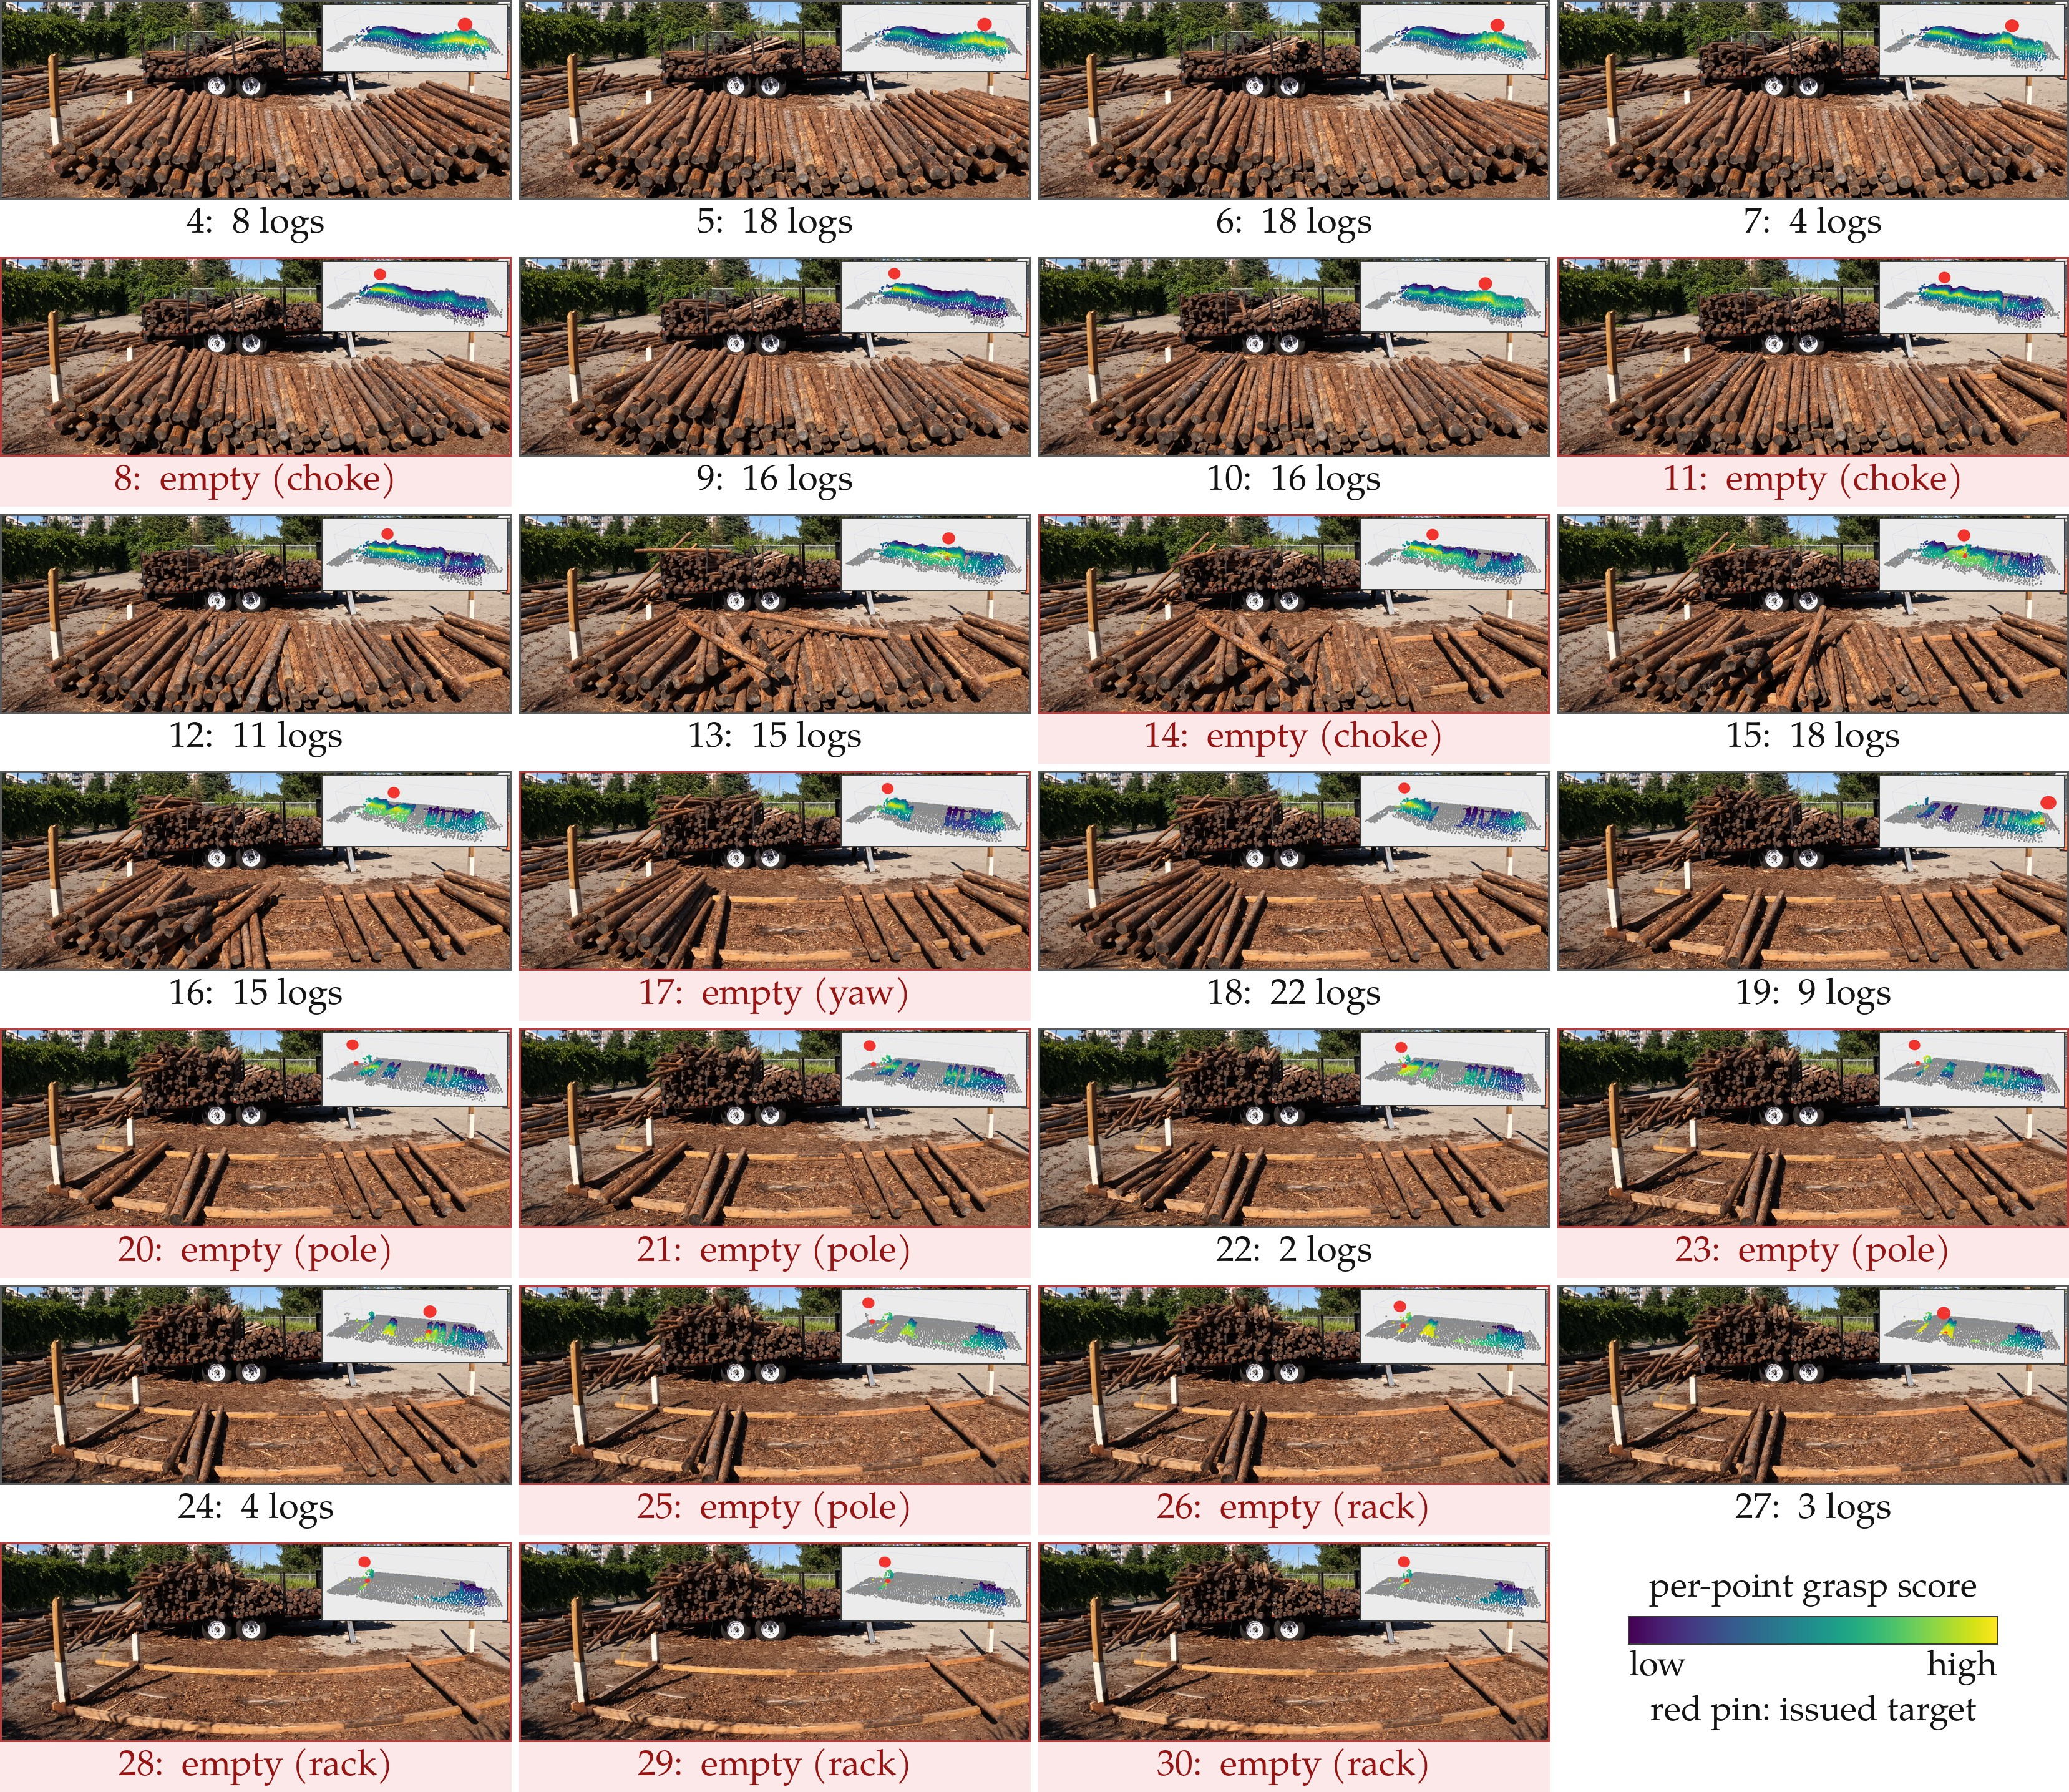
\includegraphics[width=1.12\linewidth]{figures/real_trials/clearing_grid.jpg}}
\caption{The double-mound scoring trial, one panel per grasp cycle. Each
photograph is the frame of a fixed timelapse camera at that cycle's logged
decision time; the inset is the point cloud the policy actually consumed at
that decision, colored by its per-point grasp score, with points outside the
action box (observation context, not commandable) in gray and the issued
target marked by the red pin. The cloud is drawn from the timelapse camera's
side of the rack, so left and right correspond between the photograph and the
inset. Scores are recomputed offline from the
deployed checkpoint and reproduce the logged targets. Panel labels give the
logs moved, scored from the trial record; empty cycles are tinted and
annotated with their cause. Cycles 1 to 3 preceded the start of the
recording. The rack being cleared is the ground-level bunk in the
foreground; the trailer behind it is the deposit target.}
\label{fig:bc_clearing_grid}
\end{figure}

\begin{figure}[t]
\centering
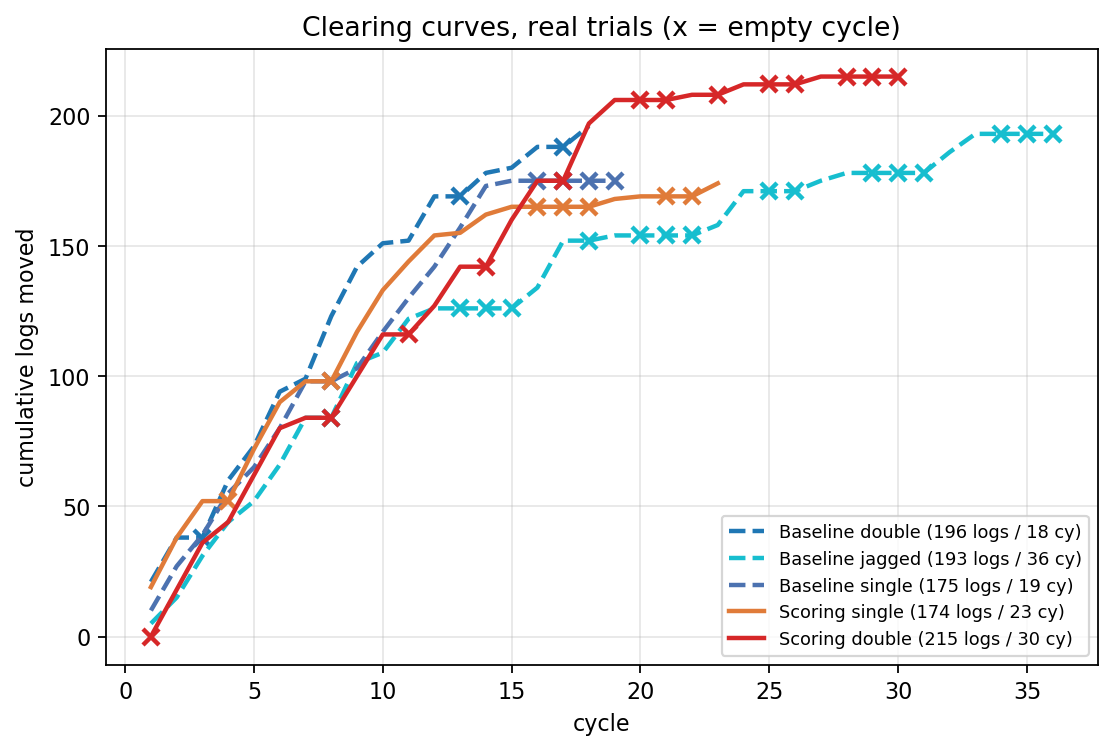
\includegraphics[width=0.92\linewidth]{figures/real_trials/clearing_curves_real.png}
\caption{Cumulative logs moved against cycle for all five trials; crosses
mark empty cycles. The baseline single-mound trial (dashed) flattens into an
unbroken run of empty cycles and was abandoned, while the scoring trials
continue to make progress through their empty cycles and finish their piles.}
\label{fig:bc_clearing_real}
\end{figure}

\begin{figure}[t]
\centering
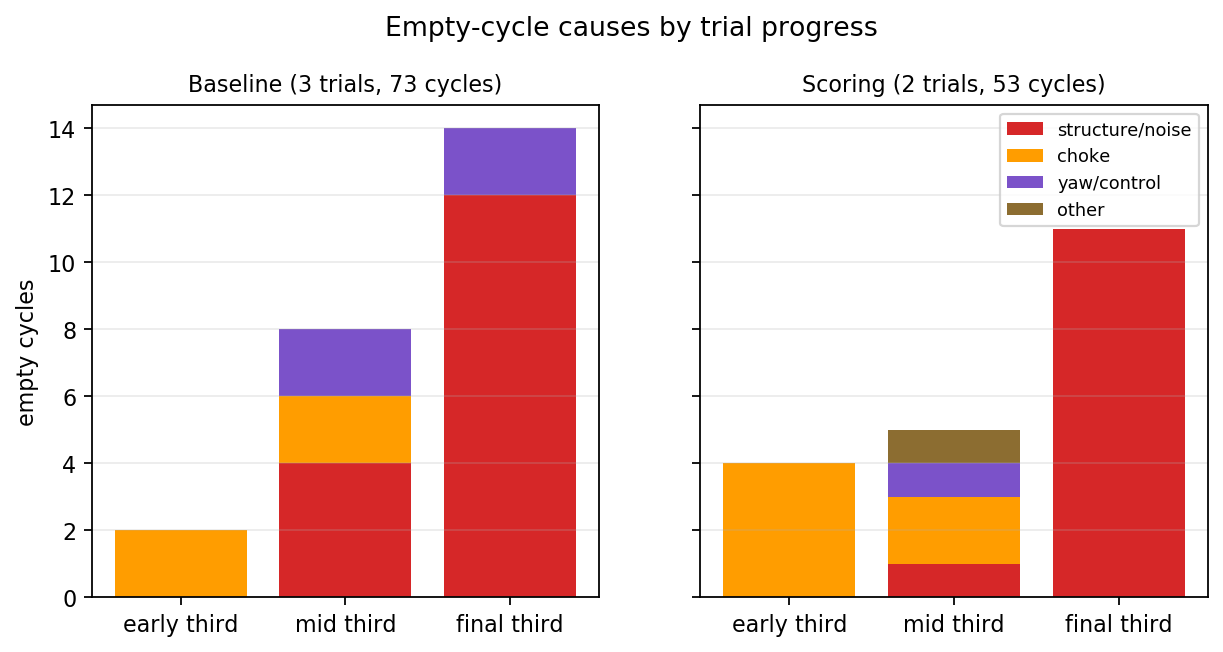
\includegraphics[width=0.92\linewidth]{figures/real_trials/failure_taxonomy_terciles.png}
\caption{Causes of empty cycles by position within the trial, pooled over the
three baseline trials (left) and the two scoring trials (right). Structure
and noise targeting concentrates in the final third for both policies, which
is where the pile falls below the rack rails; chokes are the failure class
the scoring trials added, and are a grapple-closing limit rather than a
perception error.}
\label{fig:bc_taxonomy_real}
\end{figure}

Two conclusions carry forward. The failure class that dominated the baseline
campaign and terminated trials (absorbing structure targeting) is removed or
made escapable by the scoring policy, on hardware, with the gate off, and the
gap-targeting failure of the regression policy did not occur in 30 cycles on
the shape that reliably induced it. The remaining failure classes are a depth
convention (chokes on steep mounds) and endgame structure discrimination in
the end-of-rack region, both addressable in training rather than architecture.

\section{Summary}

Both policies clone the same privileged expert from the same point-cloud
observations with the same trunk and optimizer. The regression policy is the
simpler estimator: one global feature, one 5D vector, one MSE loss. It is
accurate on unimodal scenes but, as the conditional mean, it averages when
the expert's behavior is multimodal, and on the crane that produces an
absorbing grasp-over-the-gap failure. The scoring policy replaces the
coordinate regression with a classification over observed points plus local
depth and yaw regression at the selected point. It is mode-seeking by
construction, keeps its targets on observed material, decouples target
selection from depth conventions, and admits a label-preserving translation
augmentation the regression parameterization cannot exploit, at the cost of
one piece of inference-time admissibility processing the regression policy
does not need: a candidate mask restricting the argmax to the action box.

The field evidence supports the design. The baseline campaign identified
absorbing structure and noise targeting as the dominant real failure mode
(22\% of all cycles, concentrated in the endgame), and the deployed scoring
policy either avoided it or escaped it on hardware: an unassisted full clear
on the shape that had forced the baseline to be abandoned, and zero
gap-targeting cycles on the shape that had reliably induced the regression
policy's mode-averaging failure. What remains is a depth convention (chokes
on steep mounds) and residual endgame discrimination at the end of the rack,
both training-data problems rather than parameterization problems.
